\section{Algoritmo Exacto}

\subsection{Enunciado}
En este ejercicio se nos solicita buscar el conjunto dominante mínimo y óptimo dado un grafo cualquiera. Este es un problema del tipo NP completo 
para el cual aún no se encontró forma de resolverlo polinomialmente pero tampoco se demostró que no sea posible solucionarlo con dicha complejidad.

\subsection{Soluci\'on}
Como todavía no se halló algoritmo alguno para resolverlo polinomialmente y nosotros no somos investigadores/iluminados (aún) decidimos resolverlo
de manera exponencial. Para esto utilizamos el popular método de backtracking (dicho en criollo) de quedarme con la mejor opción entre poner o no un nodo en el 
conjunto dominante. Este procedimiento lo que hace, básicamente, es analizar todas las soluciones posibles y agarrar la mejor de ellas.  \\
No nos pareció significativo agregarle memorization ya que su complejidad no mejoriría de forma considerable debido a que la complejidad del algoritmo reside en calcular cada solución posible y no en el recalculo de las mismas, además de que ocuparía mas memoria. Tampoco nos pareció imperante preocuparnos por la complejidad de la función que chequea si el conjunto recibido es dominante, ya que, mientras sea polinimal, va a ser despreciable al lado de la complejidad de analizar todas las soluciones (que como dijimos es exponencial). \\
Finalmente queremos resaltar que cualquier optimización conocida para este algoritmo no haría mas que mejorar la complejidad para ciertos tipos de casos, como el ejercicio no especifica que los grafos a recibir cumplan ciertos parametros o restricciones, todo tipo de perfeccionamiento que le implementemos va a dar lo mismo para las consignas del ejercicio.

\subsection{Pseudocódigo}

global grafoOriginal

\begin{codebox}
\Procname{$\proc{obtenerConjuntoDominanteMinimo}$ (\textbf{in} $Grafo$)}{conjuntoDom}{Conj}
\li	c = crearConj()
\li	grafoOriginal = Grafo
\li	\textbf{return} buscarMinimo(Grafo,c)
\end{codebox}

\begin{codebox}
\Procname{$\proc{buscarMinimo}$(\textbf{in} $Grafo$, \textbf{in} $conjuntoDom$)}{conjuntoDom}{Conj}
\li\textbf{Si} esDominante(conjuntoDom) \textbf{Hacer:} \Do
\li		\textbf{return} conjuntoDom 
\End
\li	\textbf{Si no}  \Do
\li		vertice = grafo.obtenerVertice(); 
\li		grafo = grafo.sinUno(vertice);
\li		conjunto1 = buscarMinimo(grafo, conjuntoDom);
\li		if($|$conjunto1$|$ == 1) \textbf{return} conjunto1
\li		conjunto2 = buscarMinimo(grafo, conjuntoDom + vertice);
\li		if($|$conjunto2$|$ == 1) \textbf{return} conjunto2
\li		\textbf{return} min(conjunto1, conjunto2)	
\End

\end{codebox}

\begin{codebox}
\Procname{$\proc{esDominante}$(\textbf{in} $Grafo$, \textbf{in} $conjuntoDom$)}{esDominante}{Boolean}
\li Grafo grafoDom = crearGrafo()
\li \textbf{Para} cada v en conjuntoDom \Do
\li	grafoDom.agregarVertice(v)
\li     grafoDom.agregarVertices(v.adyacentes())
\End
\li \textbf{Para} cada v en V(grafoOriginal) \Do
\li \textbf{Si} grafoDom.esta?(v) \textbf{Hacer:} \Do
\li			continue 
\End		
\li \textbf{Si no}  \Do						
\li		\textbf{return} false
    \End		
	\End
\li	\textbf{return} true

\end{codebox}

\subsection{Análisis de Complejidad}

La complejidad de mi algoritmo es de $2^n$ * $n^2$. Ya que hace $2^n$ recursiones y en cada una de ellas ver si el conjunto formado es dominante cuesta a lo sumo $n^2$. Voy a demostrar por inducción la parte exponencial:\\

\underline{Caso Base:}\\

n = 1, si n tiene un solo nodo ver si es dominante me cuesta O(1) ya que recorrer los vertices del grafo original es una sola iteracion y no es posible recorrer sus aristas. Luego divido en el caso en el que uso a ese nodo en el conjunto dominante y el caso en que no. El caso en que no al no tener mas nodos con cual probar me va a devolver el grafo original y el otro caso también ya que el grafo original era el que contenía únicamente a ese nodo. Ambos casos ver si el conjunto es dominante cuesta O(1) ya que tiene a lo sumo una iteración para hacer. Por lo tanto el algoritmo costaría O(1) que es igual a O($2^1*1^3$).\\

\underline{Hipótesis inductiva:}\\

Supongo que con n nodos la cantidad de recursiones es $2^n$ \\

\underline{Paso inductivo:}\\

Quiero ver que con n+1 nodos la cantidad de recursiones será $2^{n+1}$\\

Ver si el conjunto vacío es dominante me cuesta O(1) ya que en la primera iteración del grafoOriginal no es posible encontrar ningún vertice en el conjunto dominante o adyacente a él. Luego obtengo un nodo del grafo (grafo en el que me guarde todos los vertices, no el origianl) y busco el minimo conjunto dominante agregando ese nodo al conjunto o no, esto por hipótesis inductiva me cuesta 2 * ($2^n$), ya que tengo que calcular 2 veces el conjunto dominante mínimo para n nodos. Por lo tanto la complejidad me termina costando  $2^{n+1}$. Con lo cual queda demostrada la complejidad.\\
\\
Ahora voy a demostrar que verificar si el conjunto recibido es dominante cuesta  O($n^2$):\\
\\
 Esta función cuenta con 2 iteraciones, una sobre el conjunto de nodos dominantes y otra sobre el grafo original. La iteracion sobre el conjunto dominante crea un grafo con todos los nodos del conjunto y sus adyacentes, para esto agrega cada elemento del conjunto y todos sus adyacentes al nuevo grafo (obviamente si se agrega 2 veces el mismo queda 1 vez sola en el grafo) esto nos puede dar un total de n*(n-1) iteraciones, lo que pertenece a O($n^2$).\\
En la iteracion sobre el grafo original, por cada nodo de este se fija si pertence al grafo recien creado, chequear si el nodo pertence al grafo cuesta O(n) ya que debe compararlo contra todos los nodos del otro grafo y como el grafo original tiene n nodos nos terminar quedando tambien una complejidad de O($n^2$).\\
Finalmente obtenemos que la complejidad de esta verificacion es de O(2$n^2$) que es igual a O($n^2$). Por lo tanto la complejidad total del algoritmo nos termina quedando O($2^n$*$n^2$)\\


\subsection{Peor Caso}

Como el algoritmo es exacto y recorre todas las soluciones posibles siempre obtiene la mejor de ellas. Por lo tanto no existe una 'peor' instancia
en la que la solución devuelta sea sub-óptima, siempre devuelve la mejor. 

\subsection{Tests y análisis}
Como no podiamos correr el algoritmo para grafos de muchos nodos, no solo por una cuestion temporal sino porque se hace casi imposible de graficarlos por los saltos cada vez mas grandes que se producen, se nos ocurrio correr el algoritmo para grafos aleatorios. Como generamos estos grafos aleatorios? mediante un algoritmo (se encuentra en la clase grafoFactory) que recibe un n (cantidad de nodos) y un entero (probabilidad)  que lo que hace basicamente es crear un grafo con n nodos y para cada par de nodos genera un numero random de 0 a 100 y si ese numero es menor a la probabilidad recibida crea la arista entre esos nodos.\\
Como a nuestro algoritmo le agregamos que si encuentra algun conjunto dominante de un 1 nodo lo devuelva (ya que no puede haber un conjunto dominante de menos de un nodo) al aumentar el parametro probabilidad que recibe nuestro algoritmo aumentamos la probabilidad de que haya algun nodo con grado (n-1) y por lo tanto disminuimos la cantidad de ciclos de nuestro algoritmo exacto, ya que al probar el conjunto dominante con ese nodo lo devolvera automaticamente.\\
En los siguientes grafos podemos ver que a menor probabilidad mas se acerca la curva a la funcion O($2^n$*$n^2$), debido a que no encuentra un punto de corte el algoritmo y analiza todas las posibilidades, en camibo a medida que se aumenta la probabilidad la curva no solo se aleja de la funcion sino que empieza a perder su forma exponencial y aparecen casos extranos en los que un grafo de x nodos requiere menor o la misma cantidad de ciclos que un grafo de x+1 nodos. Esto se puede ver claramente en el grafo de probabilidad 50 en los puntos 14 y 15, esto pudo haberse debido a que en el grafo de 14 nodos tuvo que analizar mas casos hasta llegar al conjunto dominante de 1 nodo y en el de 15 probo antes con ese conjunto (como no agarramos los nodos con algun criterio especifico nos vienen en el orden que el grafo nos los da con la funcion obtenerVertice). 

\begin {center}
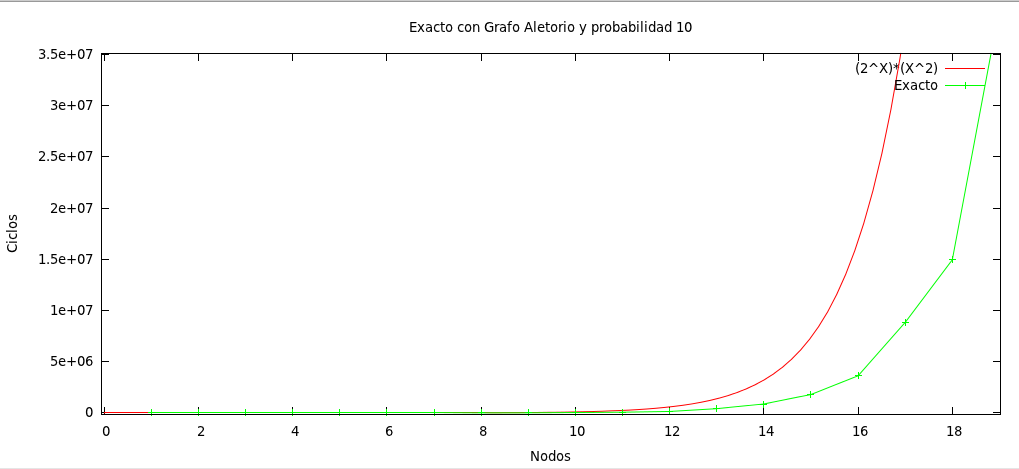
\includegraphics[width=17cm]{./graficos/exacto-proba-10.png}
% grafico.eps: 0x0 pixel, 300dpi, 0.00x0.00 cm, bb=50 50 410 302
\end {center} 

\begin {center}
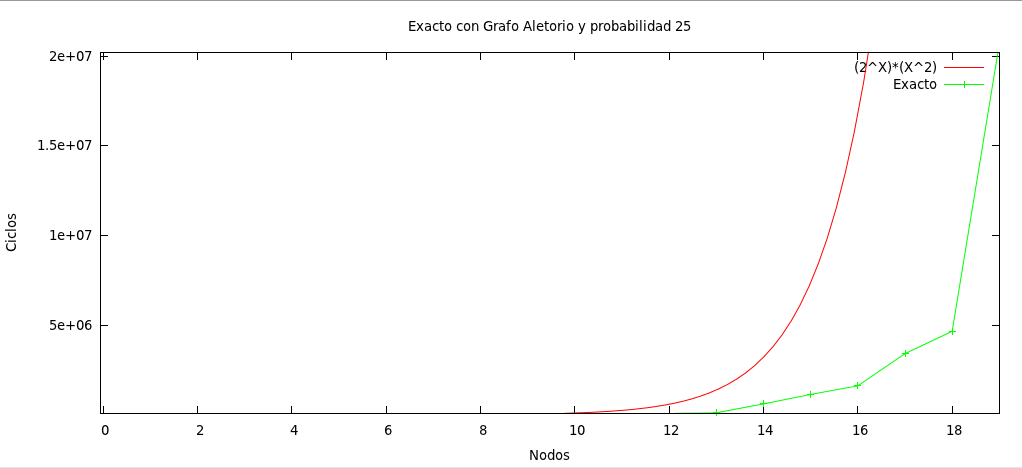
\includegraphics[width=17cm]{./graficos/exacto-proba-25.png}
% grafico.eps: 0x0 pixel, 300dpi, 0.00x0.00 cm, bb=50 50 410 302
\end {center}
 
\begin {center}
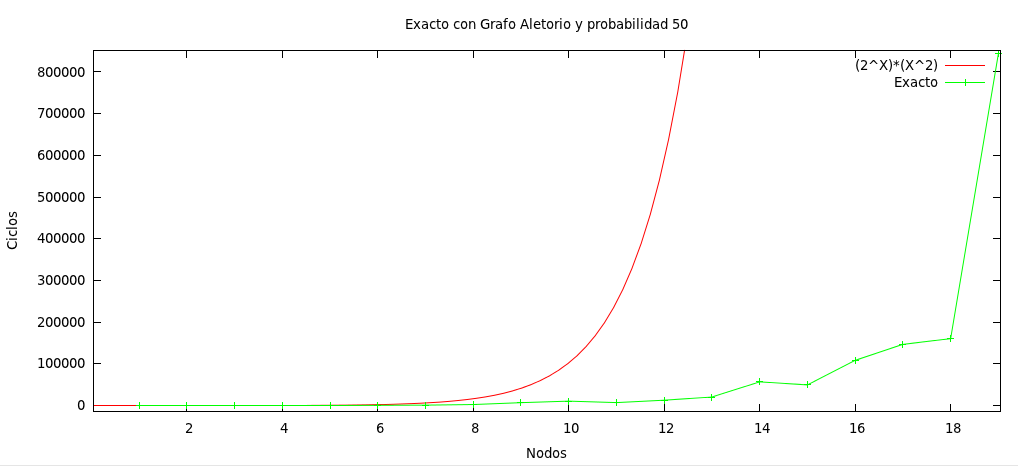
\includegraphics[width=17cm]{./graficos/exacto-proba-50.png}
% grafico.eps: 0x0 pixel, 300dpi, 0.00x0.00 cm, bb=50 50 410 302
\end {center} 
